\chapter{MapReduce}

\section{Jobs}

\subsection{Job 1: Preprocessing}

Job execution and interfaces are described in figure \ref{fig:MR-job-1}.
 
Each raw record is read and parsed into a ``Car'', i.e. a custom ``Writable'' object, during map stage. 
Each ``Car'' stores data about:
\begin{itemize}
 \item Region
 \item Price
 \item Brand
 \item Fuel
 \item Odometer
\end{itemize}

The mapper output is a pair where the key is the default one used by Hadoop when reading text files and the value is the ``Car'' itself.

The reduce stage replaces the default key with a ``NullableWritable'' so that the whole job output is a set of records yet. Then, it publishes each record several times as specified by the replication factor.

\begin{figure}[H]
	\centering
	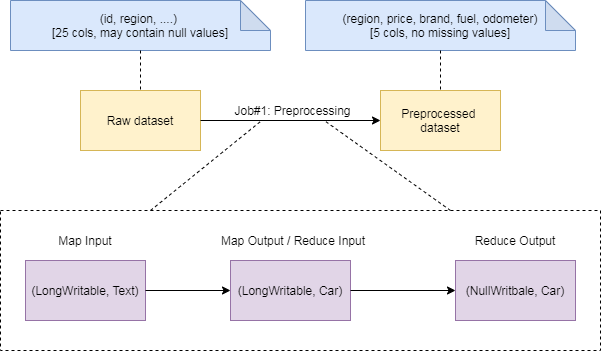
\includegraphics[scale=0.7]{images/2-mapreduce/MR-job-1.png}
	\caption{Description of ``job 1: preprocessing'' workflow and interfaces.}
	\label{fig:MR-job-1}
\end{figure}

\subsection{Job 2a: Opi}

Job execution and interfaces are described in figure \ref{fig:MR-job-2a}.

The map stage input value is a ``Car'' encoded as text. The key is the Hadoop default one (it won't be used). The mapper calculates the OPI for a given car using price and odometer fields and gives a pair consisting of (brand, OPI) as output.

The reduce stage just calculates average values using single OPIs and reports it as output.
   
\begin{figure}[H]
	\centering
	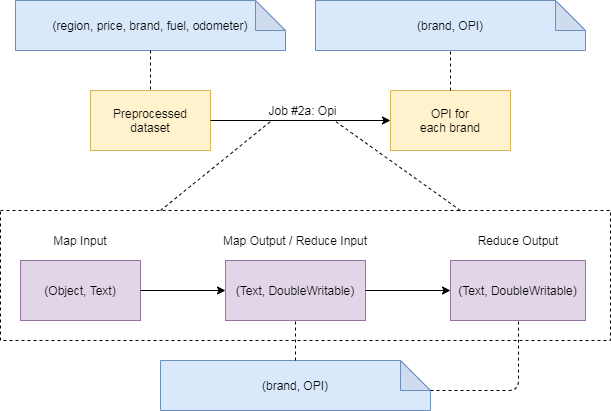
\includegraphics[scale=0.7]{images/2-mapreduce/MR-job-2a.png}
	\caption{Description of ``job 2a: opi'' workflow and interfaces.}
	\label{fig:MR-job-2a}
\end{figure}  

\subsection{Job 2b: Region}

Job execution and interfaces are described in figure \ref{fig:MR-job-2b}.

The map stage input value is a ``Car' encoded as text. The key is the Hadoop default one for text files (it won't be used). If the fuel type is correct, the mapper generates as output a pair (region, brand) so that reduce stage can operate per region basis.

The reducer, given a region, firstly calculates the cardinality for each brand by collecting the input pairs. Then, it calculates the maximum and gives it as output in the form of (region, brand).

\begin{figure}[H]
	\centering
	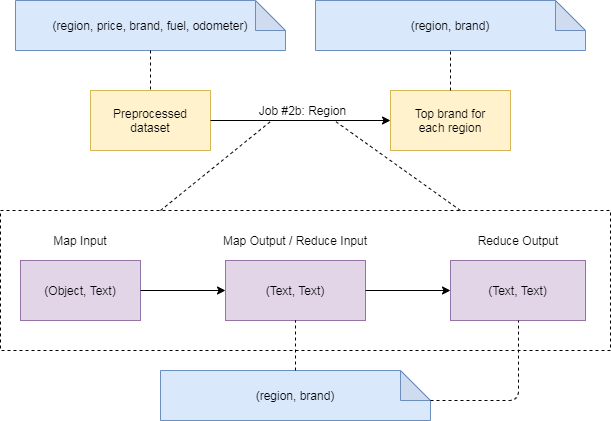
\includegraphics[scale=0.7]{images/2-mapreduce/MR-job-2b.png}
	\caption{Description of ``job 2b: region'' workflow and interfaces.}
	\label{fig:MR-job-2b}
\end{figure}  

\subsection{Job 3: Join}

Job execution and interfaces are described in figure \ref{fig:MR-job-3}.

The map stage takes as input pairs structured as (Text, Text). The source of a given pair can be from job 2a output or from job 2b output. By examinating it, it is discovered the source and the pair is marked with a flag.
Since the join key will be the brand, the output of map stage is a pair (brand, (flag, region)), where flag and region are encapsulated into a ``JoinPair'' (a custom ``Writable'').

The reducer executes the join algorithm on input items and creates output pairs in the form (region, (brand, OPI)). 

\begin{figure}[H]
	\centering
	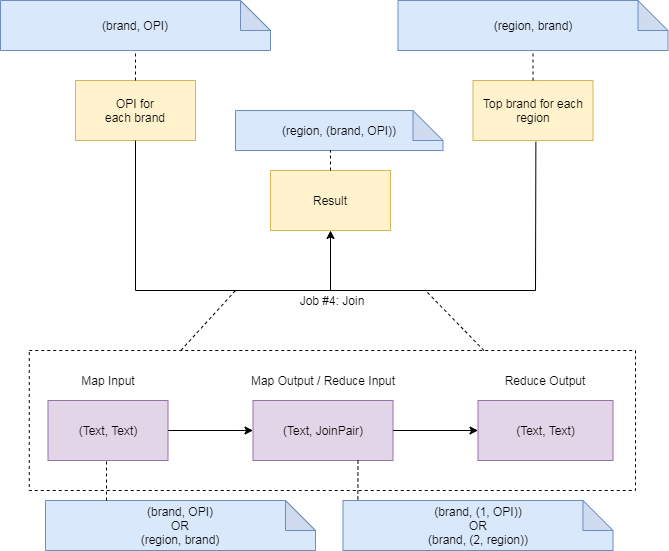
\includegraphics[scale=0.7]{images/2-mapreduce/MR-job-3.png}
	\caption{Description of ``job 3: join'' workflow and interfaces.}
	\label{fig:MR-job-3}
\end{figure}  


\section{Performance evaluation}

Performance are evaluated by varying the number of reducers, by enabling the use of combiners and by considering different replication factors.

Each casuistry result is the average value upon 3 runs. Results are shown in table \ref{table-mr-perf-100}.

As we can notice, the optimal number of reducers is 5\footnote{Actually, a more fine-grained analysis could be done by tuning the number of reducers on sigle jobs (instead of the same for each one). This could lead to find a more efficint setup but the number of combinations is quite huge and this argument will not be covered. }: too many reducers are an overkill due to task bootstrap and to the slender amount of data; on the other hand, too few reducers can't parallelize the work in the best way.

Furthermore, by compairing results in tables \ref{table-mr-perf-100} and \ref{table-mr-perf-1}, we can see that execution times for query on the bigger dataset are slightly higher than the other ones. Hence, if we consider that there are two orders of magnitude between the size of the two datasets (8.2MB against 820MB) , it is evident how such an architecture is quite an overkill for small datasets.

\begin{table}[H]
  \centering
  \begin{tabular}{ |c c|c c c c c c c| } 
    \hline
    \multicolumn{2}{ |c| }{} & \multicolumn{7}{ c| }{Reducers} \\
    \multicolumn{2}{ |c| }{} & 1 & 2 & 5 & 6 & 8 & 10 & 100 \\
    \hline
    \multirow{2}{4em}{Combiner} 
    & No  & 292 & 244 & 223 & 235 & 251 & 280 & 1235 \\      
    & Yes &  &  &  &  &  &  & \\ 
    \hline
  \end{tabular}
  \caption{Performance results expressed as elapsed time in seconds using \textbf{replication factor = 100}.}
  \label{table-mr-perf-100}
\end{table}

\begin{table}[H]
  \centering
  \begin{tabular}{ |c c|c c c c c| } 
    \hline
    \multicolumn{2}{ |c| }{} & \multicolumn{5}{ c| }{Reducers} \\
    \multicolumn{2}{ |c| }{} & 1 & 2& 5& 10 & 100 \\
    \hline
    \multirow{2}{4em}{Combiner} 
    & No  & 223 & 162 & 168 & 216 & 1400 \\      
    & Yes &  &  &  &  &   \\ 
    \hline
  \end{tabular}
  \caption{Performance results expressed as elapsed time in seconds using \textbf{replication factor = 1}.}
  \label{table-mr-perf-1}
\end{table}